\chapterimage{estados.jpg} % Table of contents heading image
\chapter{Estados}

Un estado es una situación durante la vida de un objeto, de forma que cuando dicha situación se satisface se lleva a cabo alguna acción o se espera por un evento. El estado de un objeto se puede caracterizar por el valor de una o varias de las características de su clase, además, el estado de un objeto también se puede caracterizar por la existencia de un enlace con otro objeto. El diagrama de estados y transiciones incluye todos los mensajes que un objeto puede enviar o recibir. En un diagrama de estados, un escenario simboliza un camino dentro del diagrama. Dado que generalmente el espacio entre dos envíos de mensajes representa un estado, se pueden utilizar los diagramas de secuencia para buscar los diferentes estados de un objeto \cite{Pw5DE}.

Nuestro software posee elementos que tiene diferentes estados, para poder observar como estos estados cambian, y cuales son las condiciones de transición entre estos, de mostrará a continuación un diagrama de estados donde se resume todo esto.

\section{Diagrama de Estados}

Los diagramas de estado son un método conocido para explicar el comportamiento de un sistema. Que explican todos los estados posibles en los que puede ingresar un objeto particular y la manera en que modifica el estado del objeto, como resultado de los eventos que llegan a el. Permite identificar bajo qué pruebas se ejecuta cada uno de los procesos y en qué momento podrían tener una variación. El diagrama de estados permite visualizar de una forma ordenada la ejecución de cada uno de los procesos \cite{Pw5DE}.

La siguiente figura muestra el ciclo de vida que puede tener una solicutud a la adquisicion al apoyo alimentario el cual puede encontrarse en tres diferentes estados, REVISION, ACEPTADO,RECHAZADO. Aquel evento odetonador que provoca el cambio de estado es las Condiciones el cual envia un True o unFalse dependiendo de como lo evalue el revisor y determine si dicha solicitusd cumple los requisitos. Ahora bien, existen dos transiciones entre cada fase:
\bigskip
\begin{itemize}
	\item De estado REVISION a ACEPTADO:este cambio de estado se provoca cuando la evaluacion del revisor determina que la solicitud cumple las condiciones y da su visto bueno a dicha solicitud, asignadole al detonador Condiciones el valor de True produciendo el cambio de estado.
	
	\item De estado REVISION a RECHAZADO: es cambio entre estos estados es producido cuando el revisor determina que la solicitud enviada no cumple con las condiciones necesrias para adquirir el beneficio ya sea por falta de datos o por datos incorrectos, en dicho caso el revisor rechaza la solicitud ,asignado al detonador condiciones el valor de False, provocando el cambio de estado.
	
\end{itemize}

\begin{figure}[H]
	\centering
	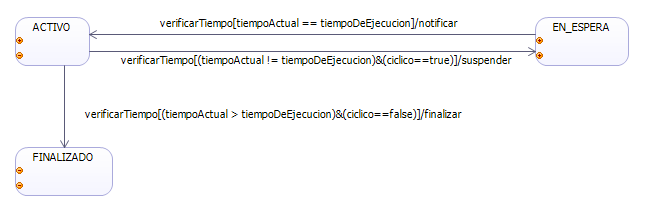
\includegraphics[width=1\linewidth]{parte2/imgs/DiagramaDeEstado/Estados}
	\caption{Diagrama de Estado}
	\label{fig:diagramaEstado}
\end{figure}

\paragraph{Diagrama de clases} 

En el siguiente esquema se muestra la clase foco que es GestionSolicitud, ésta es la que cambia de estados según las condiciones dadas, para ello debe tener como atributos un ESTADO, que es el que va a variar, y los métodos necesarios para actuar a la hora de cambiar de estado.

\begin{figure}[H]
	\centering
	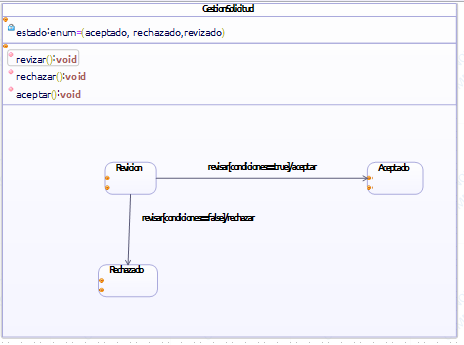
\includegraphics[width=0.8\linewidth]{parte2/imgs/DiagramaDeEstado/claseEstados}
	\caption{Diagrama de Clase Gestion de Solicitud}
	\label{fig:diagramaEstadoClase}
\end{figure}

\paragraph{Código}

El siguiente es código de nuestra clase, éste es generado por el programa de software Coloso, para la generación de éste se involucra el panorama de Java y sirve como plantilla para generar la clase correspondiente.

\begin{figure}[H]
	\centering
	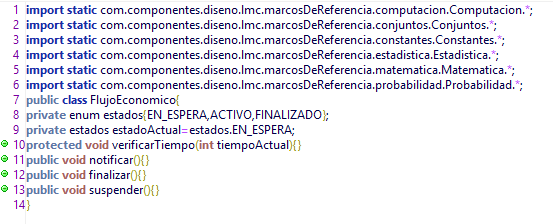
\includegraphics[width=1\linewidth]{parte2/imgs/DiagramaDeEstado/codigo}
	\caption{código de Clase Gestion Solicitud}
	\label{fig:diagramaEstadoClaseCodigo}
\end{figure}\newpage

%%%%%%%%%%%%%%%%%%%%%% Seccion 5.2 %%%%%%%%%%%%%%%%%%%%%%%%%%%%%
\section{Diagrama de flujo de trabajo}
Los diagramas de flujo de trabajo describen el comportamiento del sistema cuando tiene una actividad lo suficientemente grande para requerir un detallado de ésta, de las partes y de cómo interactuan entre sí.

Para desarrollarlo se implementan diferentes elementos como:

\begin{itemize}
	\item \textbf{Particiones}: Es una abstracción de las partes del sistema que interactua entre sí.
	\item \textbf{Actividades}: Son las tareas que le corresponde realizar a cada partición.
	\item \textbf{Transiciones}: Dan el orden en que las particiones deben desarrollar sus tareas siendo cada una dependiente de la anterior.	
	\item \textbf{Estado final}: Es el estado al que debe llegar el flujo cuando se culmine el proceso y no hayan más transiciones.
\end{itemize}

Para el software G.A.A.UD se realizo un diagrama de flujo el cual encierra las actividades fundamentales del software, iniciando desde el momento que el estudiante realiza la solicitud al apoyo alimentario hasta el momento en que es notificado si recibio dicho beneficio o no.

\paragraph{Gention de la solicitud}

 para este diagrama se requiere hacer la abtraccion de 3 paerticipantes, los cuales son el Estudiante, el Coordinador y el Revisor, iniciando desde el momento en que el estudiante realiza la solicitud, el coordinador la recive y se la envia al revisor, este la evalua luego emite dicha respuesta, la cual recive el coordinador  y segun si fue aprovada o no el coordinador le adjudicara el beneficio o no al estudiante.

\begin{figure}[H]
	\centering
	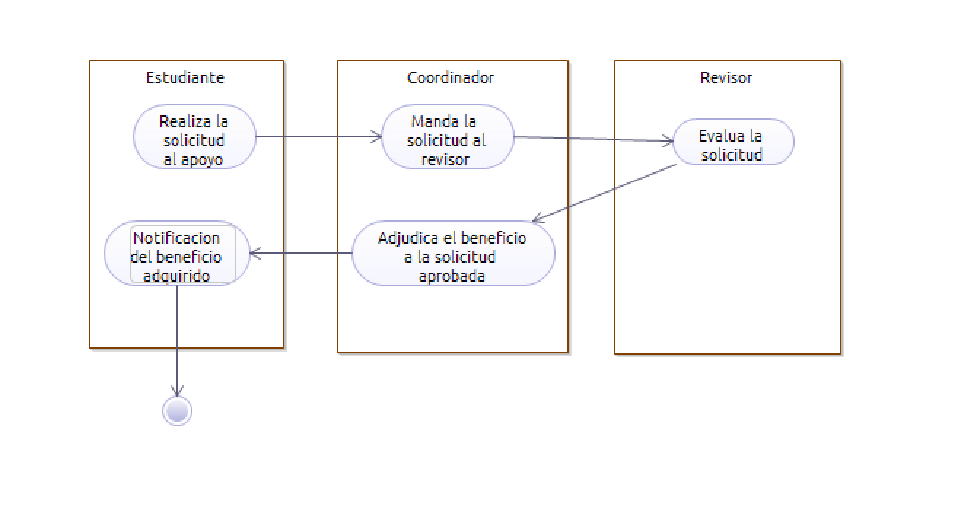
\includegraphics[width=1\linewidth]{parte2/imgs/DiagramaDeFlujoDeTrabajo/Actividades}
	\caption{Diagrama de flujo de trabajo para agregar un flujo nuevo}
	\label{fig:workflowAgregarFlujo}
\end{figure}

